% Sección 5.1
\section{Análisis y Discusión}\label{sec:analisis-discusion}

Nuestro interés en identificar y clasificar los estudios relacionados con los universos de HTCondor; que impacten en los dominios de computación distribuida y paralela, HTC, desarrollo de Software, virtualización y microservicios, redes de computadoras, infraestructura computacional, inteligencia artificial, análisis de datos, pensamiento computacional, entre otros. Que además aportan a algunos de los pilares misionales universitarios como lo es la enseñanza, la investigación y la extensión; fue enfocado hacia la creación y presentación de una taxonomía.

A través de la taxonomía propuesta, se contribuye a la organización documental de estos dominios. Ver Figura \ref{fig:taxonomia}. Una forma de usarla es facilitar la identificación y clasificación de estudios relacionados con los universos de HTCondor para fines relacionados con los de este SMS. Además, se pueden evidenciar dominios en los que se clasifican los SPS resultantes de este mapeo, lo que podría tomarse como una muestra, resultado de un proceso estructurado, de el estado del arte en torno a este tema, permitiendo así una ubicación rápida de estudios relevantes en ciertas áreas, además de un rápido resumen de algunos de los dominós relacionados con HTCondor.

\begin{figure}[htbp]
	\centering
	\vspace{10pt}
	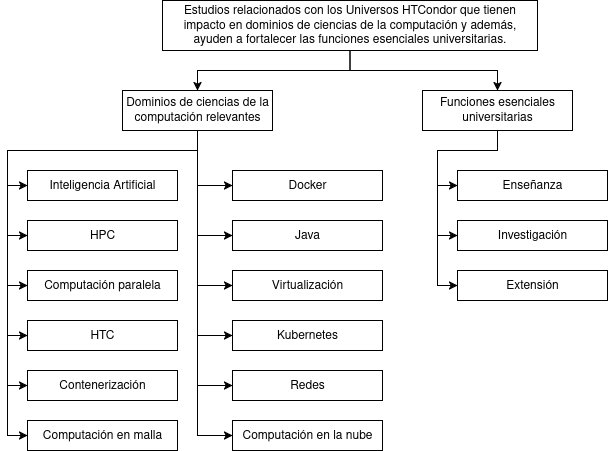
\includegraphics[scale=0.4]{resources/figures/sms-taxonomia.drawio.png}
	\vspace{6pt}
	\caption{Taxonomía de los tópicos identificados en este SMS.}
	\label{fig:taxonomia}
\end{figure}
